\section{The Cure: New Algorithms}\label{sec:algo}

In previous sections we explained from a variety of different perspectives that the Andrews-Curtis conjecture is a good example of a mathematical problem where the length of a solution can be much greater than the length of the initial presentation, in some cases with purely analytical lower bounds that are hyperexponential in the size of the input. In particular, we saw that small increases in presentation length under 20 quickly lead to solution lengths in the range of hundreds and higher, quickly exceeding the number of moves in the longest game of chess.

If solving a mathematical problem required finding a path of length $L$, say with $L=10^6$, an RL agent would be pretty much out of luck under circumstances of a typical hard search problem, where the number of successful paths is exponentially suppressed by $L$. The good news is that in mathematics --- and in many other domains --- such hard search problems never come in isolation. Rather, there is a distribution of problems such that generic instances are ``easy'' and a small fraction is ``hard.'' Learning this distribution for smaller values of $L$ contains the crucial information for solving new cases at the next increment of $L$.

\subsection{Supermoves}

In automated reasoning or search problems where the minimal length solution has a theoretical lower bound that by far exceeds computational capabilities, it is clear that direct approach with fixed size steps is not going to succeed, unless the problem is easy and a large fraction of long paths meets the desired criteria. In order to reach extraordinary path lengths, one must allow progressively longer sequences of elementary moves to be added to the action space. Although this general strategy seems unavoidable in problems like the AC conjecture, it leads to many practical questions. For example, what should be the selection criteria for such ``supermoves''? And, how often should they be added to the action space?

In the context of the AC conjecture, a good example of such supermoves are the ``elementary M-transformations'' \cite{BurnsI, BurnsII}. These transformations trivialize $\AK(2)$ in just two steps, even though this presentation is known to admit the shortest AC trivialization path of length 14. A downside of elementary M-transformations, though, is that they are infinite in number, which complicates their application in classical search techniques.

In our study, we explored the idea of identifying AC supermoves by selecting some frequently occurring subsequences of AC moves in the paths discovered by Proximal Policy Optimization (PPO). By extending the action space $A$ of the Markov Decision Process (MDP) with these subsequences and checking whether this enhanced action space helps our agent discover shorter paths of trivialization, we learned a few useful lessons:

\begin{itemize}

\item First, it helps to augment the action space with subsequences of different kind that include frequently occurring compositions of elementary moves as well as very rare ones.

\item  Also, in the early stage it helps to introduce several supermoves at once.

\item And, at later stages it helps to allow removing actions from the action space, not only adding them.
    
\end{itemize}

\noindent
Not following these empirical rules, e.g. introducing too few supermoves initially or too many over the entire length of the training process, leads to considerable reduction in performance of the RL agent. Even in the most optimal regimes that we were able to find, the improvement of the performance due to supermoves was rather modest, leading us to explore other alternatives.

\begin{figure}
	\centering
	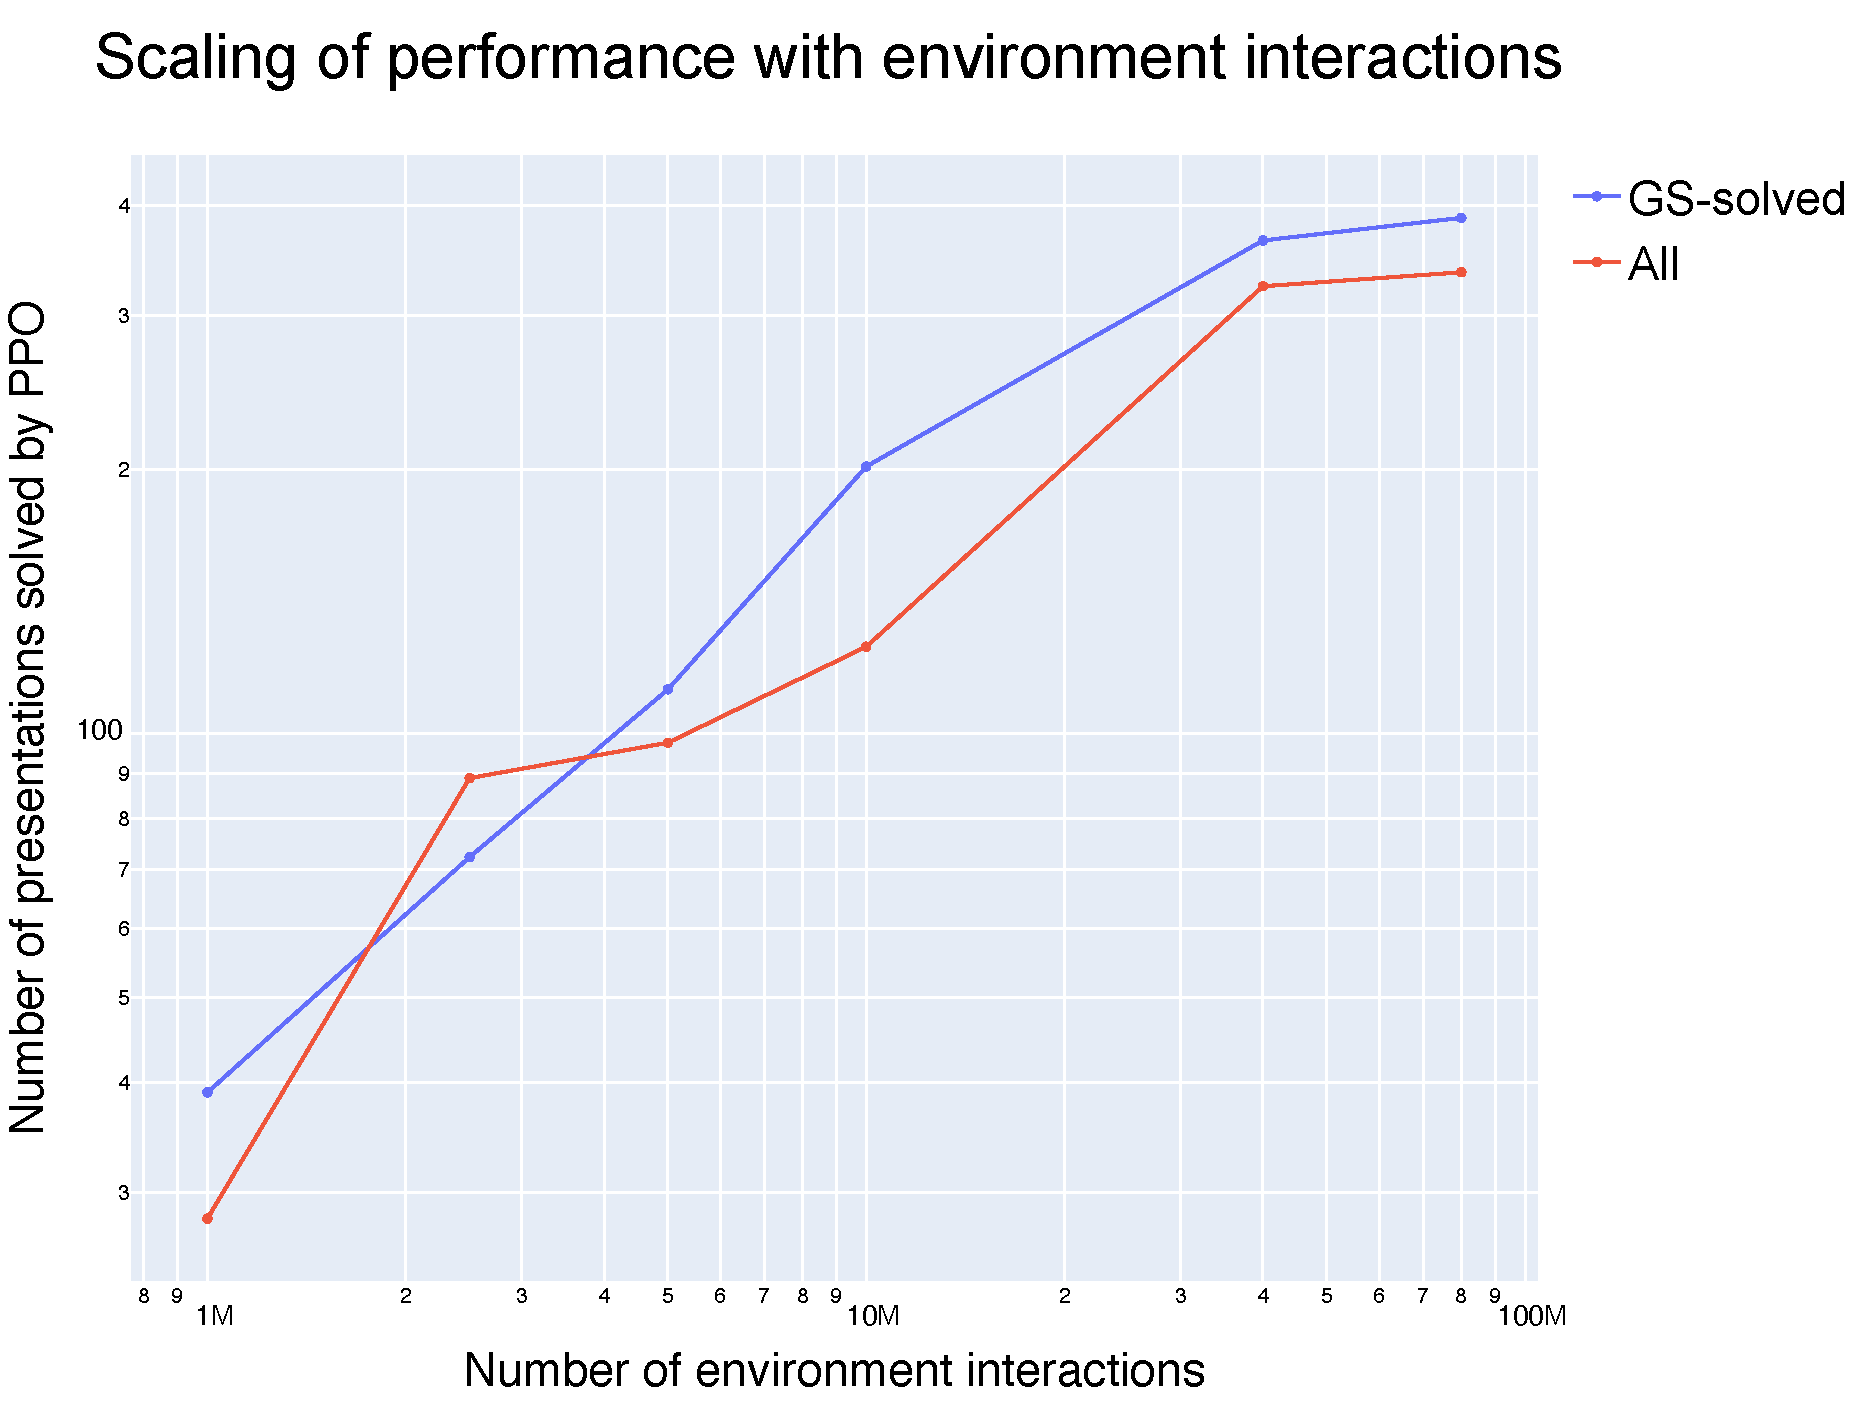
\includegraphics[scale=0.35]{fig/scaling_env.pdf}
	\caption{Number of AC presentations solved by our PPO agent as a function of the number of training steps. Here, \textit{GS-solved} refers to a subset of the Miller-Schupp dataset of \autoref{sec:search} that was solved by the greedy search algorithm.}
	\label{fig:scaling_env}
\end{figure}

\subsection{The anatomy of success}
%\subsection{New self-improving algorithms}

While supermoves clearly need to be a part of the solution in hard problems like the AC conjecture, much of the success depends on the criteria for selecting them. Here, we advocate for a dynamic approach where the network itself learns the criteria for selecting supermoves, in addition to the best ways to implement them. One realization of this approach could be a multi-agent model, where one network is learning to play the game and the other is learning the rules for changing the action space (adding and removing supermoves). We hope that future iterations of this strategy can lead to AI systems that can `learn how to learn' dynamically by making both algorithmic and architectural changes through collecting the information about hard instances.\footnote{Here, by self-improving AI systems we mean algorithms that have the ability to ``interpolate'' between off-the-shelf algorithms such as A2C and TRPO, as well as a myriad of custom algorithms that do not even have a name. Clearly, this level of technology is not presently available, and one of the key points of this section is that developing such systems should be based on the hardest instances the agent encounters.}

\begin{figure}
	\centering
	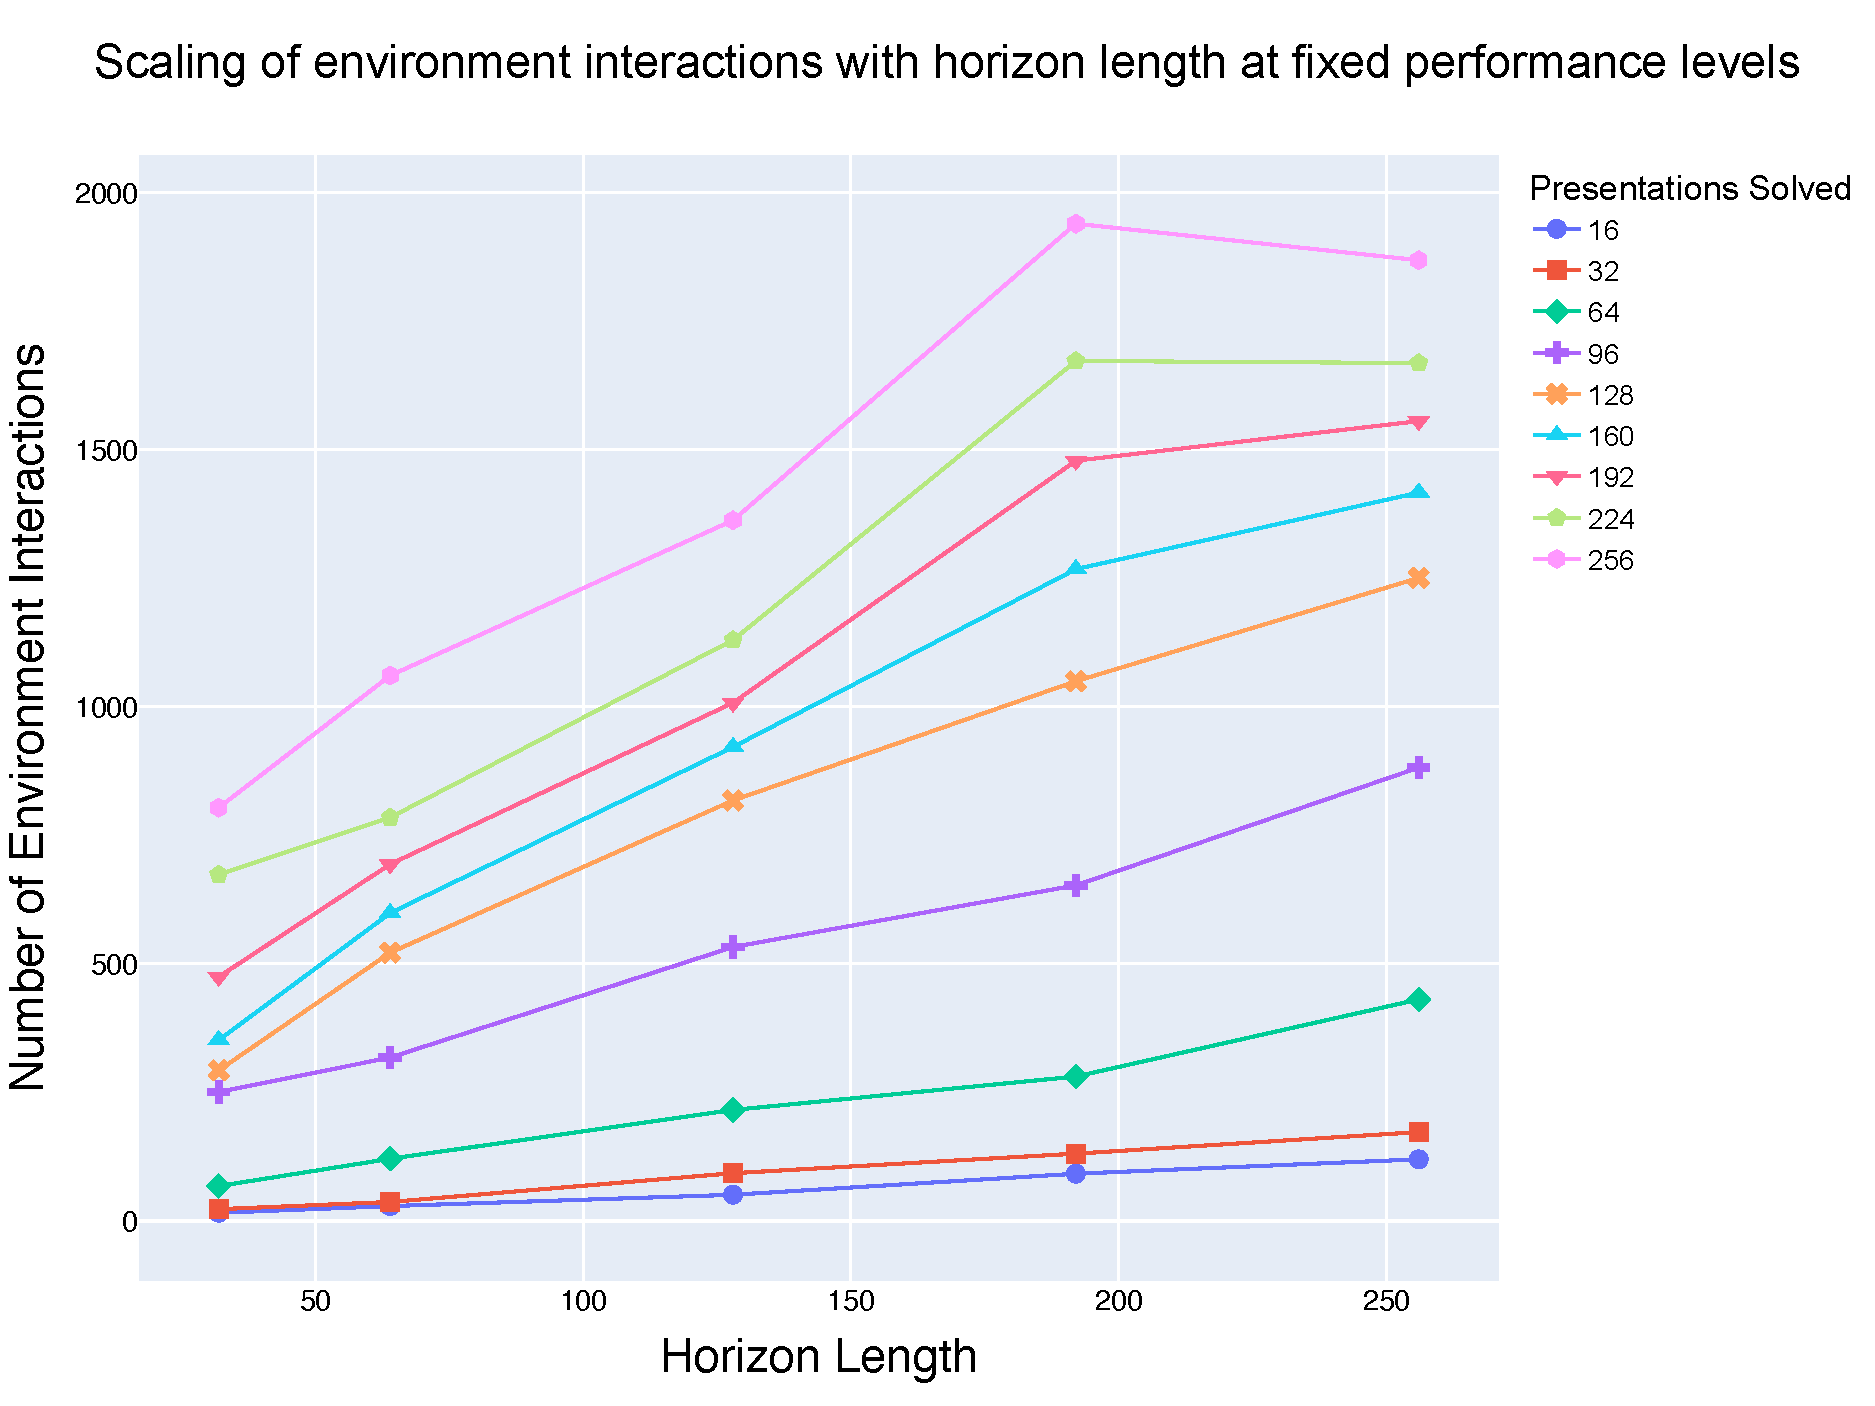
\includegraphics[scale=0.35]{fig/env_vs_horizon.pdf}
	\caption{To maintain consistent performance, increasing the horizon length requires a roughly linear increase in the number of training steps (environment interactions).}
	\label{fig:env_vs_horizon}
\end{figure}

Specifically, suppose $N$ is one of the characteristics of either the algorithm or the architecture that has non-trivial impact on performance. In practice, there can be several such parameters, but for simplicity we explain the idea as if there is only one.\footnote{Analyzing a multi-dimensional landscape is generally a good idea, as it can yield better performance improvements, but the price to pay is that changes of different characteristics become correlated, as illustrated in \autoref{fig:env_vs_horizon}.} Then, from the practical standpoint, a natural notion of hardness is such that \textit{hard instances} are defined to be those which the model can solve at the current setting of $N$ and not with the lower value of the resource $N$. In addition, in search problems we include the length of the path in the notion of hardness, i.e. select a subset of the instances that the model could solve through especially long paths. Note, by the very nature of the search problem we are interested in, there can not be too many such hard instances at each step of increasing $N$, for otherwise the problem would be easy, not hard. Collecting the information about the hardest instances at each increment in $N$ can be used to select supermoves, e.g. as subsequences of the sequences of moves that solve the hard instances. \autoref{alg:adaptive_ai_model} provides one particular realization of this idea.

\begin{algorithm}
	\caption{Adaptive AI Model Training and Path Discovery}
	\label{alg:adaptive_ai_model}
	\begin{algorithmic}[1]
		\State \textbf{Input:}
		\begin{itemize}
			\item[] Family of AI models $\pi(N)$ with common state space $S$ and action space $A_0$
			\item[] Initial setting $N_0$ and ordered range $\{N_1, N_2, \ldots, N_{\text{max}}\}$
			\item[] Number of epochs for training
			\item[] Validation set $V \subset S$
			\item[] Distinguished state $s_0 \in S$
			\item[] Positive integer $n$
		\end{itemize}
		
		\State \textbf{Output:}
		\begin{itemize}
			\item[] For each setting $N_i$: Set of pairs $\{v, P\}$ where $v \in V$ and $P$ connects $v$ to $s_0$
		\end{itemize}
		
		\State Initialize $A(N_1) \gets A_0$
		
		\For{each $N_i$ in $\{N_1, N_2, \ldots, N_{\text{max}}\}$}
		\State Train model $\pi(N_i)$ on $S$ for the given number of epochs
		\State Evaluate $\pi(N_i)$ on $V$ to discover paths connecting $V$ to $s_0$ using $A(N_i)$
		
		\State $V(N_i) \gets \{ v \in V \mid v$ can be connected to $s_0$ using $A(N_i)$, but not by any $\pi(N_j)$ with $j < i\}$
		\State $W(N_i) \gets \{ v \in V(N_i) \mid$ the longest path connecting $v$ to $s_0$ using $A_0 \}$
		
		\If{$i \geq n$}
		\State Compare $W(N_{i-n+1})$ to $W(N_i)$
		\State Adjust $A(N_{i+1})$ based on the comparison
		\Else
		\State $A(N_{i+1}) \gets A(N_i)$
		\EndIf
		\EndFor
	\end{algorithmic}
\end{algorithm}

In the context of the AC conjecture, examples of the metric $N$ can be the horizon length or the number of interactions with the environment. As \autoref{fig:scaling_env} illustrates, increasing the number of environment interactions leads to a larger number of non-trivial presentations from the Miller-Schupp series being solved (i.e. AC-trivialized). Moreover, the length of the AC trivialization path also grows for some of the solutions (but not all).
%
Therefore, in order to implement the program outlined above in the specific context of the AC conjecture, we can focus on the longest AC trivialization paths that the model is able to find at each value of $N$.

\begin{figure}[h]
    \centering
    \begin{subfigure}{0.45\textwidth}
        \centering
        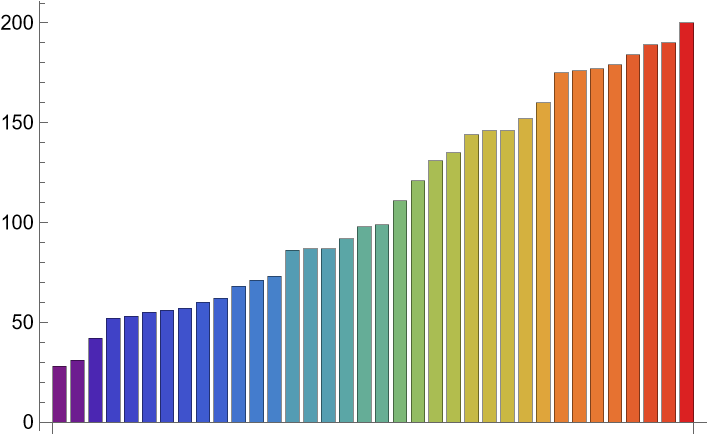
\includegraphics[width=\textwidth]{fig/all_path_length_80M.png}
        \caption{all}
        \label{fig:all_path_length_80M}
    \end{subfigure}
    \hfill
    \begin{subfigure}{0.45\textwidth}
        \centering
        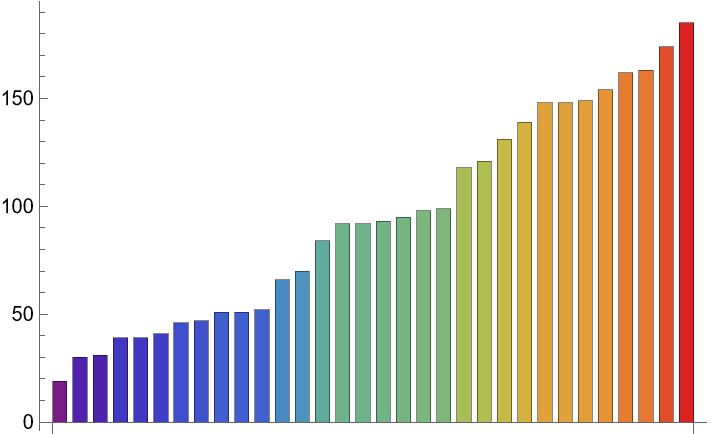
\includegraphics[width=\textwidth]{fig/solved_path_length_80M.png}
        \caption{solved}
        \label{fig:solved_path_length_80M}
    \end{subfigure}
    \caption{Path length distributions for AC presentations solved at $N=80$M from \textit{all} and \textit{solved} datasets are nearly identical. In both cases, hard instances are shown in red.}
    \label{fig:path_length_80M}
\end{figure}

Collecting this information in the process of training can be used to introduce (and remove) supermoves to the action space in a dynamic fashion. There can be many different implementations of this idea that we plan to explore more fully elsewhere. For example, one can consider selecting all or subset of the longest AC trivialization paths that the model finds at each $N$. Out of those, in each case, one can consider selecting the entire trivialization path or a subset, randomly or non-randomly. Alternatively, one can compare the longest trivialization paths at several (consecutive) values of $N$ and choose subsequences of moves that are shared by several long trivializaion paths at different $N$.

For example, if $N$ denotes the number of interactions with the environment, we did a few preliminary experiments with the dataset of \autoref{sec:rl} and several different seed values. To illustrate the effects of stochastisity, let us consider $N=80$M. The agents with five different seed values were able to solve 354, 337, 330, 328, and 323 presentations, respectively. And their average, $334.4$, is shown in \autoref{fig:scaling_env}. Many of these AC presentations can be solved at the earlier stage, with $N=40$M or less. If in the definition of \textit{hard instances} we require that they are solved by \textit{all} five agents, there are only 5 presentations total. On the other hand, if we require that they are solved by \textit{any} of the 5 agents, the number goes up to 36.

\begin{figure}[h]
    \centering
	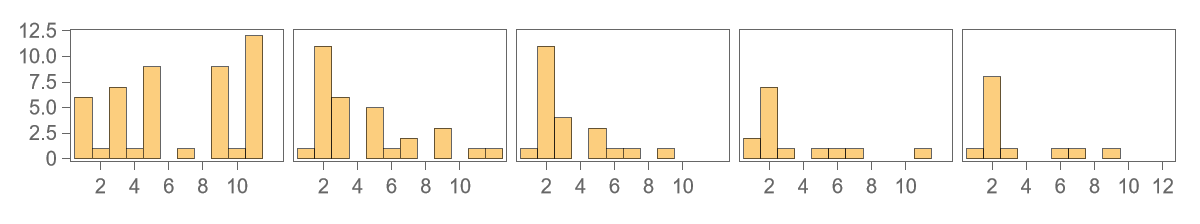
\includegraphics[scale=0.6]{fig/anatomy_all.png}
	\caption{Types of AC moves that appear in trivialization paths of 5 presentations solved by all 5 agents at $N=80$M. The move $\# 2$ occurs disproportionately more frequently. There are 12 different types of basic AC moves described in \autoref{sec:search}.}
	\label{fig:anatomy_all}
\end{figure}

Moreover, not surprisingly, the 5 presentations solved by all 5 agents have considerably shorter path lengths --- 47, 31, 22, 14, and 13 --- compared to path lengths of the 36 presentations illustrated on the left panel of \autoref{fig:path_length_80M} that go up to $200$. Both 5 presentations solved by all agents and 36 presentations solved by at least one of the agents provide viable options for defining hard instances and, in turn, selecting supermoves. However, they lead to qualitatively different results. For example, all 5 presentations solved by all 5 agents are solved at a smaller value of $N$ when required to be solved by only one of the agents. More importantly, they have very different anatomy, illustrated in \autoref{fig:anatomy_all} and in \autoref{fig:anatomy_some}, respectively.
%
By examining the longest trivialization paths of the 36 presentations solved by at least one agent at $N=80$M, we often see long strings of moves $\# 5$ and $\# 11$, interlaced with moves $\# 3$, $\# 7$, and $\# 9$. These are our top candidates for the supermoves to be added at $N=80$M.
%
Note that moves $\# 4$ and $\# 8$ are least common in the examples presented in both \autoref{fig:anatomy_all} and \autoref{fig:anatomy_some}.

\begin{figure}[h]
    \centering
	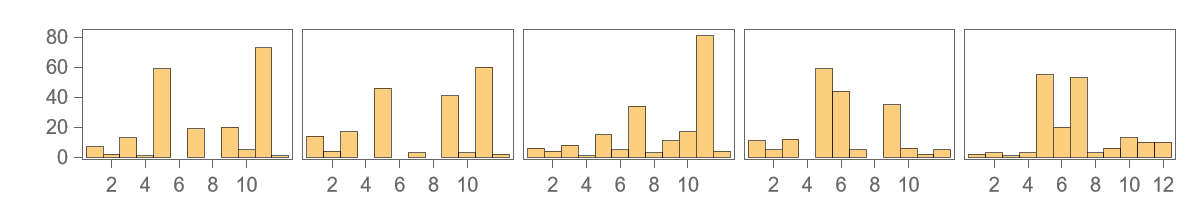
\includegraphics[scale=0.6]{fig/anatomy_some.png}
	\caption{Types of AC moves in the 5 longest trivialization paths --- of length 200, 190, 189, 184, and 179 --- found by at least one agent at $N=80$M. The most frequent moves are $\# 5$, $\# 7$, $\# 9$, and $\# 11$. There are 12 different types of basic AC moves described in \autoref{sec:search}.}
	\label{fig:anatomy_some}
\end{figure}

As in other parts of this paper, we performed the analysis on two datasets of sizes 1190 and 533 that, respectively, contain all members of the Miller–Schupp family with $n \leq 7 \, \land \, \length(w) \leq 7$ and only those solved by the greedy search. The results are qualitatively similar, as we already saw in \autoref{fig:path_length_80M} that illustrates length distributions of the successful AC paths in the two cases. Similarly, a closer look at the anatomy of the successful paths --- successful for the RL agent --- reveals no qualitative differences between the two datasets and, importantly, consistency of our notion of \textit{hardness} based on the path length. The largest level of stochasticity that one may expect perhaps can be illustrated by an example of the presentation
\[
\angles{x, y \mid x^{-1} y^2 x y^{-3} =1 \,, \; x^{-2} y^{-1} x y^{-4} =1 }
\]
that an RL agent was able to solve at $N=40$M with 62 moves in one case and at $N=80$M with 200 moves in the other case. Despite considerable variance, in both cases successful AC paths are dominated by the move $\# 11$, interlaced with moves $\# 3$, $\# 5$, $\# 7$, and $\# 9$ according to patterns described above (cf. \autoref{fig:anatomy200}). This can serve as evidence for robustness of the supermove selection process proposed here.

\begin{figure}[h]
    \centering
	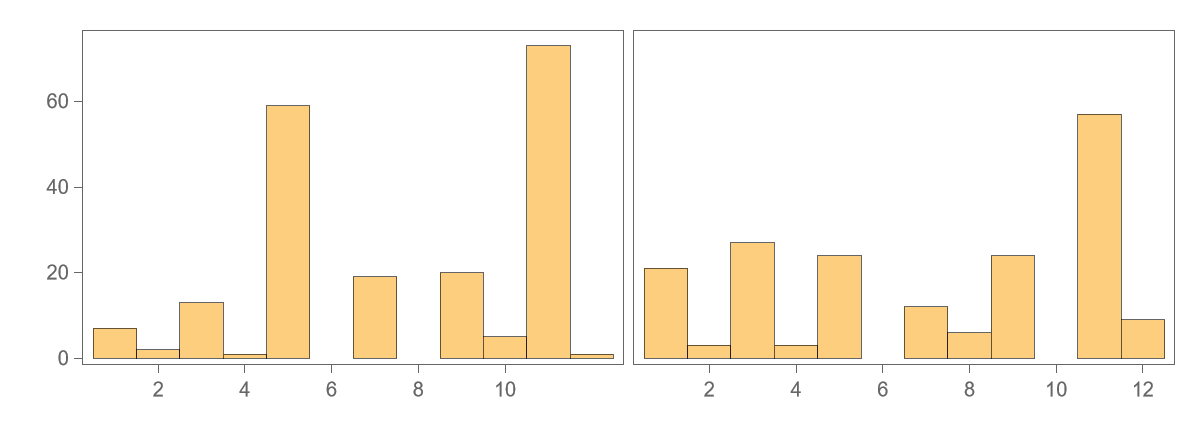
\includegraphics[scale=0.55]{fig/anatomy200.png}
	\caption{An example illustrating anatomy of successful AC paths found by an RL agent in different runs working on different datasets, both of which contain the same hard instance. Even though the total number of moves can vary, e.g. in this example we had to rescale one of the distributions by a factor of 3, curiously, the proportion of moves and combinations used are quite similar. In both cases, RL agents used the same opening move.}
	\label{fig:anatomy200}
\end{figure}

In the following sections we explore the anatomy of successful AC paths further using the tools of unsupervised learning and topological data analysis. These tools offer a complementary perspective on hard-to-find AC paths and ways to find them.
